\documentclass[tikz, border=10pt]{standalone}


\begin{document}


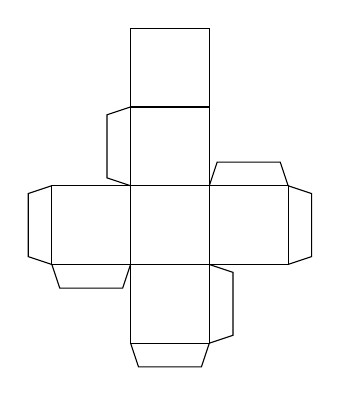
\begin{tikzpicture}[auto]
    \def\square#1#2{%
        \draw[xshift=#1cm, yshift=#2cm] (0,0) -- ++(1,0) -- ++(0,1) -- ++(-1,0) -- cycle;
    }

    \def\tab#1#2#3{
        \draw[xshift=#1cm, yshift=#2cm, rotate=#3] (0, 0) -- ++(0.1, 0.3) -- ++(0.8, 0) -- ++(0.1, -0.3);
    }

    \square{0}{0}

    \square{1}{0}
    \tab{1}{1}{0}
    \tab{2}{1}{-90}

    \square{0}{-1}
    \tab{1}{0}{-90}
    \tab{1}{-1}{180}

    \square{-1}{0}
    \tab{0}{0}{180}
    \tab{-1}{0}{90}

    \square{0}{1}
    \tab{0}{1}{90}

    \square{0}{2}
\end{tikzpicture}

\end{document}